\section{Iterative convergence and benchmark verification}
\label{suppsec:convergence}

\subsection{Iterative convergence}

Each simulation was run until the relative change of the velocity field between successive measurement windows fell below $10^{-8}$. The final residual and iteration count are recorded for every case in the scalar output files. All $24$ cases at $N=384$ in the main campaign ($N_w=1$, $\alpha\in\{0,0.1\}$) satisfied this criterion, with residuals at or below $9.9\times10^{-9}$ and $478$k--$1.21$M iterations. The convergence history for representative cases is shown in Fig.~\ref{suppfig:residual}.

\begin{figure}[!htbp]
\centering
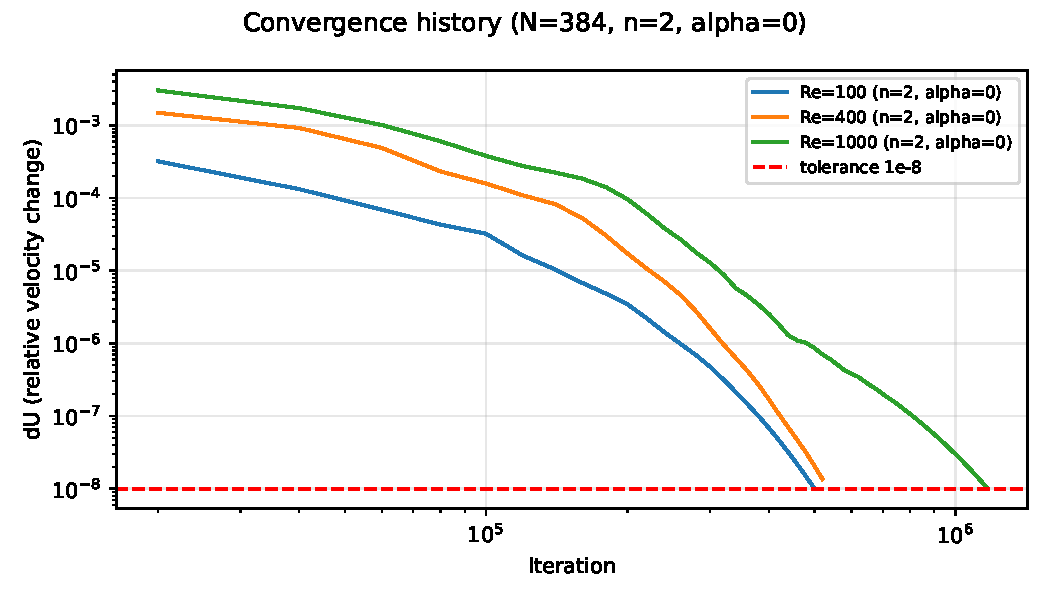
\includegraphics[width=0.8\columnwidth]{figures/figS_residual.pdf}
\caption{Iterative residual versus iteration number for representative cases at $N=384$. All cases converge to residuals at or below $10^{-8}$.}
\label{suppfig:residual}
\end{figure}

\subsection{Benchmark verification against Ghia et al.}

Two distinct comparison cases are reported, to separate the effect of the geometry from that of the lid treatment.

\emph{Exact square cavity.} An exact square cavity with a flat bottom and a \emph{uniform} (non-regularized) lid was run separately at $Re=100$, $400$, and $1000$, and $N=128$--$384$. This isolates the flat-wall and uniform-lid limits of the solver and is the case directly comparable with Ghia et al.~\cite{Ghia1982}. At $N=256$ the maximum absolute centerline deviations are $0.0062$ and $0.0102$ ($Re=100$), $0.0033$ and $0.0058$ ($Re=400$, excluding the single anomalous tabulated datum at $x=0.9063$~\cite{Chai2006}), and $0.0050$ and $0.0136$ ($Re=1000$) for $\max|u-u_G|$ and $\max|v-v_G|$; these reproduce the previously validated reference errors ($0.0057$, $0.0080$, $0.0141$). The exact-square metrics are collected in Table~IV of the main text.

\emph{Near-square campaign case.} The exact square cavity is not one of the campaign geometries; the closest available case is $n=8$, $\alpha=0$, with $A_f=0.9892$ and rounded bottom corners, and it uses the \emph{regularized} lid ($\varepsilon=0.02$) of the production solver. Its centerline profiles were compared with the same benchmark at $N=256$, using the same interior stations and the same exclusion of the anomalous $Re=400$ datum as for the exact square. The maximum absolute deviations are $0.0038$ and $0.0054$ ($Re=100$), $0.0035$ and $0.0034$ ($Re=400$), and $0.0046$ and $0.0066$ ($Re=1000$) for $\max|u-u_G|$ and $\max|v-v_G|$---of the same order as, and in several cases smaller than, the exact-square values. The curved-wall (Bouzidi) treatment and the near-square bottom therefore do not degrade the interior solution despite the regularized lid, which differs from the uniform lid of Ghia at the top corners. Neither comparison validates the energetic integrals, whose grid sensitivity is treated in Section~\ref{suppsec:consistency}. Detailed metrics are given in Table~\ref{supptab:benchmark}.

\begin{table}[!htbp]
\centering
\caption{Benchmark verification against Ghia et al.~\cite{Ghia1982}. Top block: exact square cavity (flat bottom, uniform lid), maximum absolute deviations $\max|u-u_G|$ ($x=0.5$) and $\max|v-v_G|$ ($y=0.5$) at $N=256$; the single anomalous tabulated datum at $(Re{=}400,\,x{=}0.9063)$~\cite{Chai2006} is excluded from $\max|v-v_G|$ in the final column. Bottom block: near-square campaign case $n=8$, $\alpha=0$ ($A_f=0.9892$, regularized lid), same interior stations and same exclusion.}
\label{supptab:benchmark}
\begin{tabular}{@{}lcccc@{}}
\hline
Case & $Re$ & $\max|u-u_G|$ & $\max|v-v_G|$ & excl. \\
\hline
exact square & $100$  & $0.0062$ & $0.0102$ & $0.0102$ \\
exact square & $400$  & $0.0033$ & $0.1492$ & $0.0058$ \\
exact square & $1000$ & $0.0050$ & $0.0136$ & $0.0136$ \\
\hline
$n=8$, $\alpha=0$ & $100$  & $0.0038$ & $0.0054$ & $0.0054$ \\
$n=8$, $\alpha=0$ & $400$  & $0.0035$ & $0.1425$ & $0.0034$ \\
$n=8$, $\alpha=0$ & $1000$ & $0.0046$ & $0.0141$ & $0.0066$ \\
\hline
\end{tabular}
\end{table}

\begin{table}[!htbp]
\centering
\caption{Isolating the effect of the regularized production lid on a \emph{strictly flat} square cavity ($A_f=1$). The complete $Re\times N\times$lid matrix is reported as the maximum interior-centerline deviations from Ghia et al.~\cite{Ghia1982} ($\max|u-u_G|$ / $\max|v-v_G|$), using the same interior stations and the same exclusion of the anomalous $Re=400$ datum at $x=0.9063$. The last two columns give the regularized-minus-uniform change; it never exceeds $5.5\times10^{-4}$. The lid regularization therefore removes only the corner singularity and does not measurably bias the interior flow.}
\label{supptab:lidreg}
\begin{tabular}{@{}lccc@{}}
\hline
$Re$ & $N$ & $\max|u-u_G|$ / $\max|v-v_G|$ (uniform) & $\max|u-u_G|$ / $\max|v-v_G|$ (regularized) \\
\hline
100  & 128 & $0.00754$ / $0.01091$ & $0.00752$ / $0.01092$ \\
100  & 256 & $0.00623$ / $0.01020$ & $0.00622$ / $0.01019$ \\
400  & 128 & $0.00800$ / $0.00746$ & $0.00810$ / $0.00755$ \\
400  & 256 & $0.00329$ / $0.00580$ & $0.00334$ / $0.00578$ \\
1000 & 128 & $0.01197$ / $0.01069$ & $0.01251$ / $0.01119$ \\
1000 & 256 & $0.00502$ / $0.01358$ & $0.00516$ / $0.01347$ \\
\hline
\end{tabular}
\end{table}

\subsection{Independent-solver cross-validation}
\label{suppsec:crosscheck}

As a final check that the energetic contrasts are not an artifact of the MRT-LBM discretisation, the two-member primary contrast $I_D(2,4)$ at $Re=400$, $\alpha=0$ was recomputed with a completely independent solver: a conforming Taylor--Hood finite-element method (P2 velocity / P1 pressure, Picard linearisation) on a boundary-fitted mesh graded toward the wall and the lid. The geometry function was replaced by the superelliptic wall of Eq.~\eqref{suppeq:yb} so that both solvers integrate over the identical domain, and the same regularized lid profile is imposed in both: the finite-element solver prescribes the identical cubic-smoothstep lid velocity $U(x)=U_{\rm lid}\,g(x)$ with the same corner-regularization width $\varepsilon=0.02$ used by the lattice-Boltzmann production run (a prescribed Dirichlet velocity on the top boundary for the FEM, the corresponding regularized momentum injection for the LBM). All finite-element energetics are reported \emph{natively}: the strain-rate, lid-power, and kinetic-energy integrals are evaluated element-wise from the finite-element velocity field, with no projection onto the LBM grid and no LBM wall-gradient model. The native finite-element energy balance closes to $0.01\%$ at the finest mesh ($P^*=D^*$ to $0.01\%$), and within $0.22\%$ over all meshes (Table~\ref{supptab:femconv}). The meshes $nx=ny=64,128,256$ were run for both $n=2$ and $n=4$.

The independent finite-element calculations provide a cross-solver consistency check. At the finest available resolutions the finite-element and lattice-Boltzmann dissipation contrasts differ by approximately $0.002$ percentage points ($I_D(2,4)=+0.323\%$ at $nx=256$ versus $+0.325\%$ at $N=384$). The finite-element estimates, however, span $0.023$ percentage points across the three meshes ($+0.346\%$, $+0.332\%$, $+0.323\%$ at $nx=64,128,256$), which exceeds the finest-grid FEM--LBM gap; this agreement is therefore not interpreted as evidence of finite-element convergence toward the lattice-Boltzmann value (Table~\ref{supptab:crosscheck}). The FEM calculation is reported throughout strictly as a cross-solver consistency check, at $Re=400$ and (Section below) at $Re=1000$, and never as a convergence result for either solver. On the matched finest grids (FEM $nx=256$, LBM $N=384$) the absolute levels agree to a few percent ($K^*: +1.1\%$, $D^*: +2.0\%$, $P^*: +4.1\%$), and all three contrasts agree to within $0.02$ percentage point ($I_K: 0.019$~pt, $I_P: 0.008$~pt, $I_D: 0.002$~pt). The larger $P^*$ offset combines the coarser resolution of the lid shear layer at $N=384$ with the residual $2\%$ lattice-Boltzmann power--dissipation imbalance at that grid; both are grid effects that cancel in the paired contrast, exactly as the main text argues.

\emph{Cross-check at $Re=1000$.} The two coarser meshes were also run at $Re=1000$, where the primary contrast is an order of magnitude larger than at $Re=400$. The native finite-element contrast is $+0.716\%$ at $nx=64$ and $+0.598\%$ at $nx=128$, against $+0.5909\%$ at $N=384$ in the lattice-Boltzmann production set: the finer mesh differs by $0.008$ percentage point, or $1.3\%$ in relative terms, and the sequence moves toward the lattice-Boltzmann value under refinement. The native energy balance of these runs closes to $+0.41\%$ ($n=2$) and $+0.21\%$ ($n=4$) at $nx=64$ and to $+0.16\%$ and $+0.15\%$ at $nx=128$. The $nx=256$ mesh was not attempted at $Re=1000$: a single case commits about $9$~GB for the sparse assembly, which cannot be accommodated on this node while the lattice-Boltzmann campaigns are running. The finite-element variation across its own two meshes at this Reynolds number ($0.117$ percentage point) again exceeds the finest-grid finite-element--lattice-Boltzmann gap ($0.008$ percentage point), so this second comparison is reported with the same restriction as at $Re=400$: it is a cross-solver consistency check, not an independent convergence proof for either solver.

\begin{table}[!htbp]
\centering
\caption{Independent-solver cross-validation at $Re=400$ and $Re=1000$, $\alpha=0$: Taylor--Hood FEM (native, $nx=ny=64/128/256$) versus the MRT-LBM ($N=128/256/384$). Top: mesh sensitivity of the native finite-element dissipation contrast $I_D(2,4)$ at both Reynolds numbers; the $nx=256$ finite-element mesh was not run at $Re=1000$, where the memory cost of the sparse assembly exceeds the budget available during the lattice-Boltzmann campaigns. Bottom: absolute $n=2$ reference values and the geometric contrasts, on the finest grids of each solver (FEM $nx=256$, LBM $N=384$). All finite-element entries are native (element-wise integrals, no projection); the LBM-grid-projected finite-element contrasts are $+6.1\%$ ($Re=400$, $nx=64$), $+2.0\%$ ($Re=400$, finest native mesh), $+32.6\%$ and $+11.8\%$ ($Re=1000$, $nx=64$ and $128$), and are not used in any comparison.}
\label{supptab:crosscheck}
\begin{tabular}{@{}lcccc@{}}
\hline
$nx$ & $64$ & $128$ & $256$ & LBM $N=384$ \\
\hline
$I_D(2,4)$ [\%], $Re=400$  & $+0.346$ & $+0.332$ & $+0.323$ & $+0.325$ \\
$I_D(2,4)$ [\%], $Re=1000$ & $+0.716$ & $+0.598$ & --- & $+0.591$ \\
\hline
\end{tabular}

\vspace{4pt}

\begin{tabular}{@{}lccc@{}}
\hline
Quantity (finest grids) & FEM ($nx=256$) & LBM ($N=384$) & rel.\ diff. \\
\hline
$K^*$ ($n=2$), native   & $0.040440$ & $0.040011$ & $+1.1\%$ \\
$P^*$ ($n=2$), native   & $23.899$   & $22.954$   & $+4.1\%$ \\
$D^*$ ($n=2$), native   & $23.896$   & $23.432$   & $+2.0\%$ \\
\hline
$I_K(2,4)$              & $+0.752\%$ & $+0.771\%$ & $0.019$~pt \\
$I_P(2,4)$              & $+0.321\%$ & $+0.328\%$ & $0.008$~pt \\
$I_D(2,4)$              & $+0.323\%$ & $+0.325\%$ & $0.002$~pt \\
\hline
\end{tabular}
\end{table}

\begin{table}[!htbp]
\centering
\caption{Native finite-element mesh-refinement study at $Re=400$, $\alpha=0$: absolute $n=2$ and $n=4$ values of $K^*$, $P^*$, $D^*$ and the native energy balance $P^*/D^*-1$, together with the exact mesh fluid area against the analytic superellipse area ($A_f=0.892699$ for $n=2$, $0.963519$ for $n=4$). The balance stays within $0.22\%$ at all meshes and reaches $0.01\%$ on the finest mesh, and the mesh fluid area approaches the analytic superellipse area under refinement.}
\label{supptab:femconv}
\begin{tabular}{@{}lcccccc@{}}
\hline
$n$ & $nx$ & $K^*$ & $P^*$ & $D^*$ & $P^*/D^*-1$ & $A_f^{\mathrm{mesh}}$ \\
\hline
2 & 64  & $0.040420$ & $23.804$ & $23.819$ & $-0.06\%$ & $0.891888$ \\
2 & 128 & $0.040434$ & $23.960$ & $23.908$ & $+0.22\%$ & $0.892412$ \\
2 & 256 & $0.040440$ & $23.899$ & $23.896$ & $+0.01\%$ & $0.892598$ \\
4 & 64  & $0.040702$ & $23.872$ & $23.901$ & $-0.12\%$ & $0.960547$ \\
4 & 128 & $0.040729$ & $24.038$ & $23.987$ & $+0.21\%$ & $0.962268$ \\
4 & 256 & $0.040744$ & $23.975$ & $23.973$ & $+0.01\%$ & $0.962993$ \\
\hline
\end{tabular}
\end{table}
